\chapter{システム追加実験の詳細}
\label{chap:system}
システム実験では全3回にわたる実験を行ったが追加実験ではシステムの実験の第1段階における1日目のみを実施した.
\section{被験者のデータ}
実験対象者は計22人の10代-20代学生(男性6名:女性4名)であり,システム実験と同様の事前質問を行った結果を
表\ref{table:before-extra}に示す.


\begin{table}[H]
    \caption{事前質問項目:システム実験}
    \label{table:before}
	\scriptsize
    \begin{tabular}{l||c}
        \multicolumn{1}{c|}{質問} & 回答の平均\\ \hline \hline
        ボードゲームの経験はどれくらいありますか & 2.18\\
        connect4(ゲーム)の経験はどれくらいありますか& 1.64\\\hline
        機械学習に対する知識はどれくらいありますか& 3.59\\
        強化学習に対する知識はどれくらいありますか& 3.23\\
    \end{tabular}
    
\end{table}
\section{実験設定の詳細}
AIの強さは表\ref{table:param-system}における「弱いAI」モデルを使用した.
また,システム実験における第1段階と同様に1回の実験当たりの制限時間は7分とし,実験内のAIとの対戦は2回までに制限した.

\subsection{振り返りモード(GUI)の詳細}
GUIは主にシステム実験第1段階における2日目のGUIと類似している.
ただし,図\ref{fig:extra}に示すように訪問回数「counts」の表記を廃止し,「value」と数字ボタンは「traj\&value」ボタンを
押した際に出現する.
\begin{figure}[t]
	\centering
    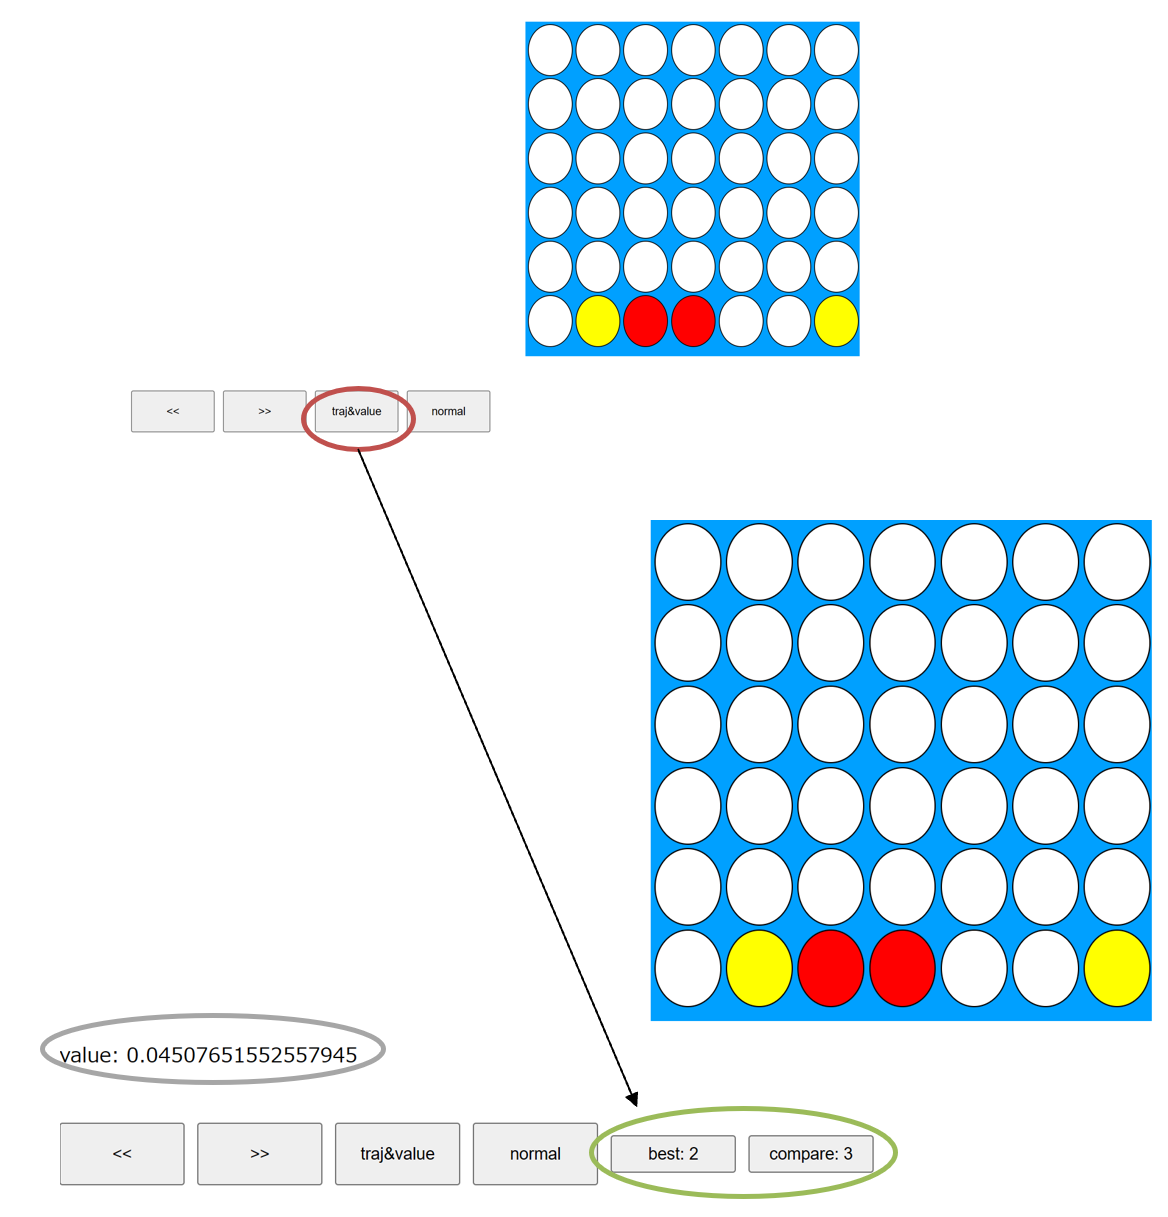
\includegraphics[width=\linewidth]{./figure/extra.png}
	\caption{GUI(追加実験)}
	\label{fig:extra}
\end{figure}

\subsection{アルゴリズムの変更}
追加実験では最も訪問回数$N(s, a)$が大きい行動$a_m$から派生する進行図と$a_m$から「最も遠い」行動$a_l$から派生する進行図と
を表示する.
「最も遠い」行動$a_l$は以下の手順によって定められる.また,アルゴリズムの疑似コードはAlgorithm\label{alg:myalg-add} に記載している.
\begin{enumerate}
    \item 盤面$s$から派生する各行動$\{a_1, a_2, ..., a_n\}$に対して提案手法または比較手法による
    軌道を収集する.その際に各行動に対して局面評価$Q(s, a)$と軌道の長さの平均$L(s, a)$を記録する.
    \item 最も訪問回数$N(s, a)$が大きい行動$a_m$による局面評価を$v(=Q(s, a_m))$とする.
    また,任意の閾値$l$に対して$\textrm{margin}_m(=l-L(s, a_m))$を計算する.
    \item 局面評価の符号が$v$と異なる行動$\{a_{d_1}, a_{d_2}, ..., a_{d_k}\}$を取り出す.
    \item $\{a_{d_1}, a_{d_2}, ..., a_{d_k}\}$内の各行動に対して$\textrm{margin}(=l-L(s, a))$を計算し,
    $\textrm{margin}$の符号が$\textrm{margin}_m$と異なる行動$\{{a'}_{1}, {a'}_{2}, ..., {a'}_{k}\}$を取り出す.
    \item 取り出した行動のうち軌道の長さの平均$L(s, a)$が$L(s, a_m)$と最も遠い行動$a_l$を最適な行動$a_m$から最も遠い行動
    とする.
\end{enumerate}
このアルゴリズムは状態$s$,最適な行動$a_m$から派生する局面評価$Q(s, a_m)$と予測される軌道の長さの平均$L(s, a_m)$が遠い行動を取り出している.
つまり,「予測される勝敗」と「あとどのくらいでゲームが終了するか」の予想がなるべく$a_m$による予想と異なるものを取り出すことを意味している.

また,第4章の図\ref{fig:regroup}に記載したように,被験者に与える情報を可能な限り少なくする目的で取り出した進行図の軌道を末尾の3手で
さらにグループ化し,提案手法において1組の状態$s$,行動$a$に対して閲覧できる進行図の数は3つまでとした.
図\ref{fig:re-regroup}に再度,再グループ化の様子を示す.
\begin{figure}[t]
	\centering
	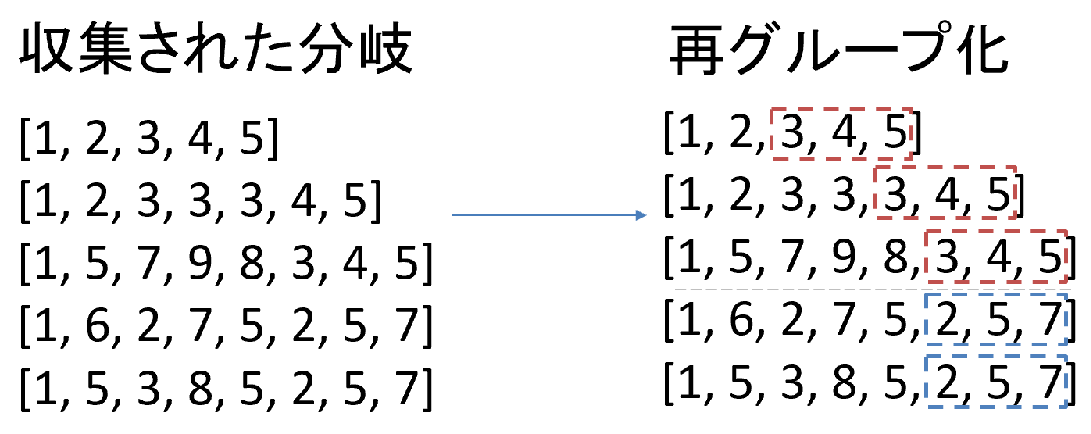
\includegraphics[width=\linewidth]{./figure/regroup.pdf}
	\caption{再グループ化(再掲)}
	\label{fig:re-regroup}
\end{figure}

\begin{algorithm}
    \small
    \caption{追加実験のアルゴリズム}
    \label{alg:myalg-add}
    \begin{algorithmic}[1]
        \State $t$: 手法を適用する探索木
        \State $T$: 状態遷移関数
        \State $l$: 任意の閾値
        \State $L(s, a)$: $(s, a)$の進行図における軌道の長さの平均

        
        
       
        \Function{ExtactDistantChoice}{$s_{start}$}
           \For {each $i$ in $\{1, 2, 3, 4\}$}
               $A_i \gets $ empty list
           \EndFor
           \State $a_m = \textrm{argmax}_a N(s_{start}, a)$
           \State $Z_m \gets$ \Call{MyAlgorithm}{$s_{start}, a$}
           \State $L_m \gets $ $Z_m$内の各軌道の長さの平均
           \State $\textrm{margin} \gets (l-L_m)$
           \State $v_m \gets Q(s, a_m)$
           \State $A \gets \{a_1, a_2, ..., a_n\}$ ($A$は$s_{start}$から派生する行動の集合)
           \For {each $a_i$ in $A$}
            \State $Z_i \gets$ \Call{MyAlgorithm}{$s_{start}, a_i$}
            \State $L_i \gets $ $Z_i$内の各軌道の長さの平均
            \State $\textrm{margin}_i \gets (l-L_i)$
            \If{$Q(s, a_i) \times v_m < 0$}
                \If{$\textrm{margin}  \times \textrm{margin}_i < 0$}
                    \State $A_1$に$a_i$を追加
                \Else
                    \State $A_2$に$a_i$を追加
                \EndIf
            \Else
                \If{$\textrm{margin}  \times \textrm{margin}_i < 0$}
                    \State $A_3$に$a_i$を追加
                \Else
                    \State $A_4$に$a_i$を追加
                \EndIf

            \EndIf
           \EndFor

           \For {each $i$ in $\{1, 2, 3, 4\}$}
                \If{$A_i$の要素数が1以上}
                   $A_0 \gets A_i$
                \EndIf
           \EndFor
           \State $d \gets 0$
           \State $a_l \gets \textrm{argmax}_a (|L(s,a)-L_m|)$
           \State \Return $a_l$
        \EndFunction
    \end{algorithmic}
\end{algorithm}












\section{質問項目の詳細}
質問項目は表\ref{table:query}に記載した質問に加え,「タスクの熟達度に関連する質問」として「振り返りでは対戦を振り返るのに十分な量の情報を受け取ることができたと思いますか」
という質問を追加した.
\section{結果データ}
第4章では先読みの手数ごとに結果データを集計した.ここでは他の観点から集計されたデータを示す.
表\ref{table:system-all}に先読みの手数を分けずに合計した結果を示す.
\begin{table}[H]
    \caption{結果:総合}
    \scriptsize
    \centering
    \resizebox{\linewidth}{!}{
        \begin{tabular}{c|l||c|c}
            \multicolumn{2}{c}{質問} & \multicolumn{2}{c}{主観評価} \\ \hline \hline
            質問の種類 & 質問の内容 & A & B \\ \hline 
            (a) & 振り返りによって成長したと感じましたか & 3.55 & \bf{3.86} \\
            & 振り返りによってAIの意図を掴むことができたと感じますか & 2.73 & \bf{3.32} \\
            & (2回目のみ) 1回目に比べて成長したと感じますか & 3.36 & \bf{4.00} \\ \hline
            (b) & 今後も connect4 をプレイするときにこのシステムを使いたいと思いましたか & 4.05 & \bf{4.27} \\
            & システムにより振り返りが楽しくなったと感じますか & 3.86 & \bf{4.33} \\
        \end{tabular}
    }
    \label{table:system-all}
\end{table}

また,AIの強さごとに集計した結果を表\ref{table:system-strong},表\ref{table:system-weak}に示す.
表\ref{table:system-strong}に強いAIを用いて訓練した被験者のデータ,表\ref{table:system-weak}に
弱いAIを用いて訓練した被験者のデータを示す.
\begin{table}[H]
    \caption{結果:AIの強さ(強い)}
    \scriptsize
    \centering
    \resizebox{\linewidth}{!}{
        \begin{tabular}{c|l||c|c}
            \multicolumn{2}{c}{質問} & \multicolumn{2}{c}{主観評価} \\ \hline \hline
            質問の種類 & 質問の内容 & A & B \\ \hline 
            (a) & 振り返りによって成長したと感じましたか & 3.67 & \bf{3.82} \\
            & 振り返りによってAIの意図を掴むことができたと感じますか & 2.58 & \bf{3.55} \\
            & (2回目のみ) 1回目に比べて成長したと感じますか & 3.00 & \bf{4.00} \\ \hline
            (b) & 今後も connect4 をプレイするときにこのシステムを使いたいと思いましたか & 4.08 & \bf{4.64} \\
            & システムにより振り返りが楽しくなったと感じますか & 3.75 & \bf{4.50} \\
        \end{tabular}
    }
    \label{table:system-strong}
\end{table}

\begin{table}[H]
    \caption{結果:AIの強さ(弱い)}
    \scriptsize
    \centering
    \resizebox{\linewidth}{!}{
        \begin{tabular}{c|l||c|c}
            \multicolumn{2}{c}{質問} & \multicolumn{2}{c}{主観評価} \\ \hline \hline
            質問の種類 & 質問の内容 & A & B \\ \hline 
            (a) & 振り返りによって成長したと感じましたか & 3.8 & \bf{3.33} \\
            & 振り返りによってAIの意図を掴むことができたと感じますか & 3.00 & 3.00 \\
            & (2回目のみ) 1回目に比べて成長したと感じますか & 3.80 & \bf{4.00} \\ \hline
            (b) & 今後も connect4 をプレイするときにこのシステムを使いたいと思いましたか & \bf{4.00} & 3.80 \\
            & システムにより振り返りが楽しくなったと感じますか & 4 & \bf{4.1} \\
        \end{tabular}
    }
    \label{table:system-weak}
\end{table}
また,1日目のデータを表\ref{table:system-day1},2日目のデータを表\ref{table:system-day2}に記載する.
\begin{table}[H]
    \caption{結果:1日目}
    \scriptsize
    \centering
    \resizebox{\linewidth}{!}{
        \begin{tabular}{c|l||c|c}
            \multicolumn{2}{c}{質問} & \multicolumn{2}{c}{主観評価} \\ \hline \hline
            質問の種類 & 質問の内容 & A & B \\ \hline 
            (a) & 振り返りによって成長したと感じましたか & 3.56 & \bf{3.78} \\
            & 振り返りによってAIの意図を掴むことができたと感じますか & \bf{3.05} & 2.94 \\ \hline
            (b) & 今後も connect4 をプレイするときにこのシステムを使いたいと思いましたか & 4.06 & \bf{4.28} \\
            & システムにより振り返りが楽しくなったと感じますか & 4.06 & \bf{4.28} \\
        \end{tabular}
    }
    \label{table:system-day1}
\end{table}

\begin{table}[H]
    \caption{結果:2日目}
    \scriptsize
    \centering
    \resizebox{\linewidth}{!}{
        \begin{tabular}{c|l||c|c}
            \multicolumn{2}{c}{質問} & \multicolumn{2}{c}{主観評価} \\ \hline \hline
            質問の種類 & 質問の内容 & A & B \\ \hline 
            (a) & 振り返りによって成長したと感じましたか & 3.55 & \bf{3.91} \\
            & 振り返りによってAIの意図を掴むことができたと感じますか & 2.45 & \bf{3.64} \\ 
			& (2回目のみ) 1回目に比べて成長したと感じますか & 3.36 & \bf{4.00} \\ \hline
            (b) & 今後も connect4 をプレイするときにこのシステムを使いたいと思いましたか & 4.00 & 4.18 \\
            & システムにより振り返りが楽しくなったと感じますか & 3.91 & \bf{4.40} \\
        \end{tabular}
    }
    \label{table:system-day2}
\end{table}


